\documentclass[   
state        = Report,                       % (Report | Slide    | Thesis)
lang         = EN,                           % (DE     | EN) 
degree       = MSc,                          % (BSc    | MSc)
dept         = MECH,                         % (MECH   | SBT)
bib-active   = true,                         % (true   | false)
bib-style    = ieee,                         % (ieee)
column-type  = two,                          % (one    | two)
]{mcidoc}

% CUSTOM COMMANDS -----------------------------------------------------------------------------
%       
% Please enter any custom command/packages you require here for easy tracking 
\usepackage{float}

% For example, bibliography setting are added. Bibtex is the standard but if you prefer
% there are other options on the market such as biber. Style has been chosen as IEEE but if 
% are from another discipline, please feel free to change it.

\bibliography{references.bib}  % Here we add our file where we store our references.
%      
% ---------------------------------------------------------------------------------------------
 
% DOCUMENT PARAMETERS -------------------------------------------------------------------------

\TitleHeader{Project Report}%   

\Title{%
  Parallel Kinematics of a Delta Robot
}% 

\Lecture{Robotics}%    

\Lecturer{Mehmet Ismet Can Dede, PhD}%

\Cohort{MA-MECH-25-VZ}%           
\Group{H}%

\StudentName{Andreas Thöni}%
\StudentID{2510620039}% 

%\Supervisor{Colin Stevens}%

\begin{document} % ############################################################################

\MakeTitlePage     

\TableOfContents           

% REPORT CONTENT ------------------------------------------------------------------------------

% ----      
% Your report content should go here and should follow structure befitting of a scientific
% report and should be written in a scientific format. For more information please look at
% MCI guidelines on how it should be done.      
% ----  

% Include Chapter - introduction
%\chapter{Task description}

The task of this project was to generate a model for the Delta 360 parallel manipulator by \textsc{IGUS} in \textsc{MATLAB} using the \textsc{Simscape} Multibody blockset. After generating the model, several \textsc{MATLAB} functions should be implemented to compare theoretical calculations of kinematics with the simulation, move in joint- and task-space, and create suitable trajectories.



   

% chaptas
\chapter{Task description}

The task of this project was to generate a model for the Delta 360 parallel manipulator by \textsc{IGUS} in \textsc{MATLAB} using the \textsc{Simscape} Multibody blockset. After generating the model, several \textsc{MATLAB} functions should be implemented to compare theoretical calculations of kinematics with the simulation, move in joint- and task-space, and create suitable trajectories.




% !TeX root = ../Main-Report.tex

\chapter{Simscape Multibody Modeling}

The Multibody model of the robot has been created using the \textsc{Simscape Multibody Link Plugin} and several files that have been given by the lecturer. Using the plugin, it is possible to create a simulation from an exported .xml file and several .step-files, both exported from CAD-software, in this case from \textsc{Solidworks}. The resulting model has then been slightly adjusted to be usable for the tasks at hand. These adjustments include:

\begin{itemize}
	\item the addition of a transform sensor, which is able to measure the relative transform between the origin of our chosen coordinate system and the end-effector.
	\item the addition of several transform adjustments, to ensure the correct detection of the relative transform.
	\item the addition of position input ports to the prismatic joints, to be able to control them accordingly.
	\item the addition of three subsystems, which automatically compute the first two derivatives of the input position information and perform a sign-correction.
\end{itemize}

A screenshot of how the adjusted model looks can be seen in figure \ref{fig:mbmodeldelta}.

\begin{figure}[H]
	\centering
	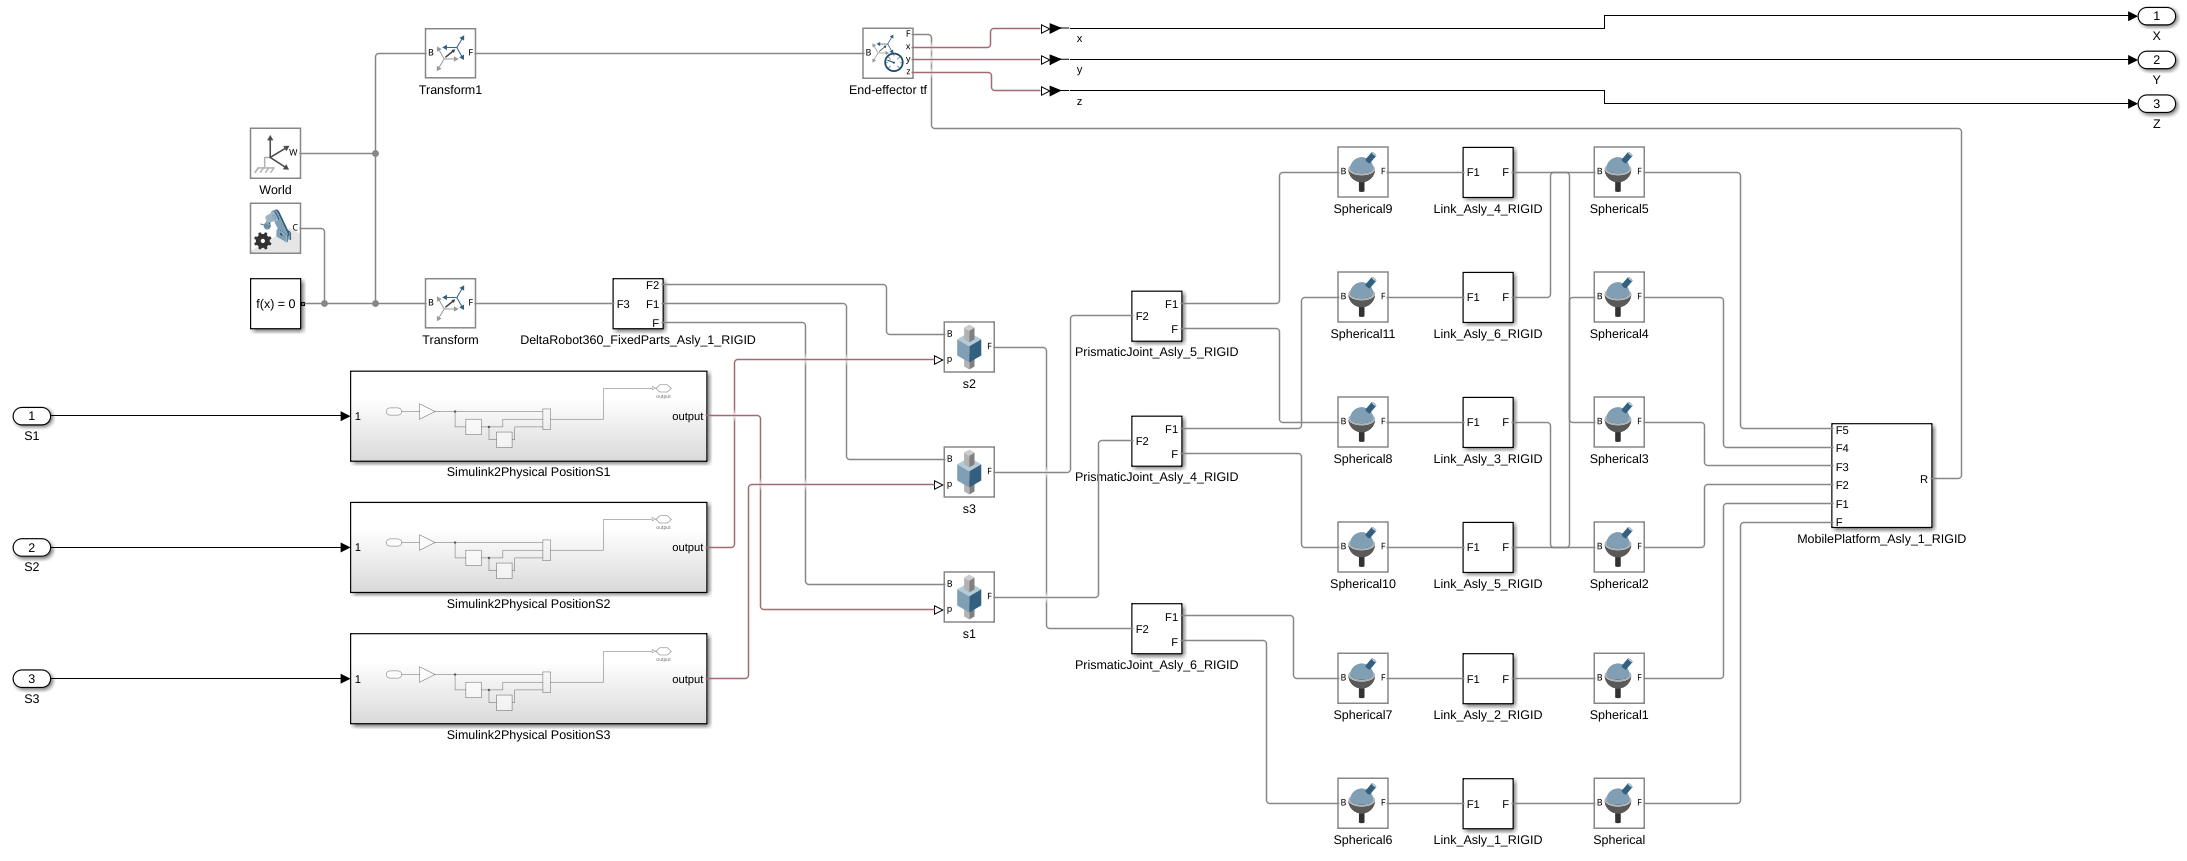
\includegraphics[width=1.0\linewidth]{cus_imgs/MB_model_delta}
	\caption{Adjusted Simscape Multibody model of the robot}
	\label{fig:mbmodeldelta}
\end{figure}

% !TeX root = ../Main-Report.tex

\chapter{Forward and Inverse Kinematics}


\section{Forward Kinematics}
Calculating forward kinematics is the process of determining the endeffector position depending on the joint variables. The equations for calculating the forward kinematics as well as the needed dimensions of the Delta robot have been taken from \cite{delta_kin} and were put inside a MATLAB-function block to be usable inside Simulink. The code of the function block can be found in \textit{forward\_kinematics.m}.

To be able to verify if the equations have been implemented correctly, the euclidean error between the Multibody simulation (MB) and the output of the forward kinematics function (FK) has been calculated. The results can be seen in figure \ref{fig:fwkinverification}.

% TODO: \usepackage{graphicx} required
\begin{figure}[H]
	\centering
	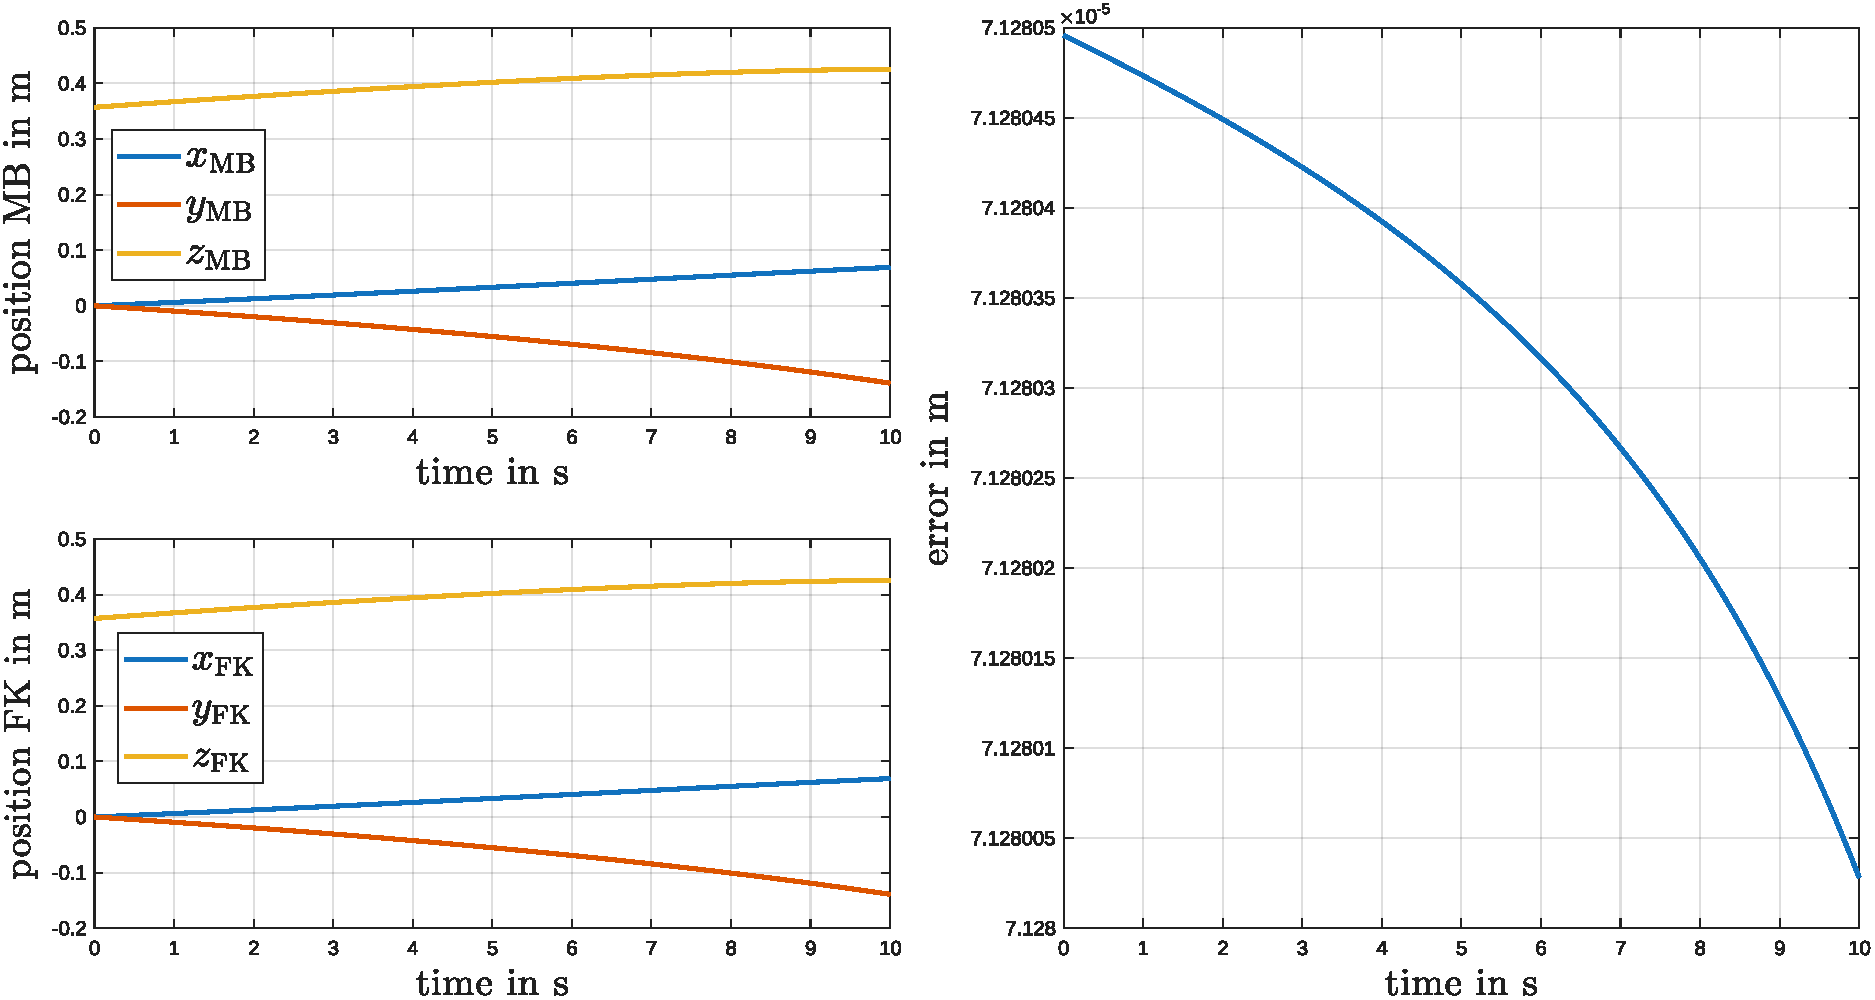
\includegraphics[width=1.0\linewidth]{cus_imgs/fw_kin_verification2}
	\caption[Plot of verification process for forward kinematics]{Plot of Verification process for forward kinematics. Left column: position calculated by Multibody model (MB) and function (FK); right column: euclidean error of the two}
	\label{fig:fwkinverification}
\end{figure}

The left column shows that for the joint trajectory that has been given to the system, the position of the end-effector in simulation and the forward kinematics function yield the same result. The plot in the right column shows an error of magnitudes of $10^{-5}\,\si{\meter}$, which is neglectable.

\section{Inverse Kinematics}
Calculating inverse kinematics is the process of determining the joint positions necessary for the end-effector to be at a given position. The equations for inverse kinematics for the robot are also taken from \cite{delta_kin}. A function called \textit{inverse\_kinematics.m} has been implemented to do the conversion. To verify the results, the end-effector output of the  Multibody-model has been fed into the inverse kinematics function, whose output has been compared to the input into the Simulation. Like above, the inputs are three ramps with different inclinations. The results can be seen in figure \ref{fig:inkinverification}.
\begin{figure}[H]
	\centering
	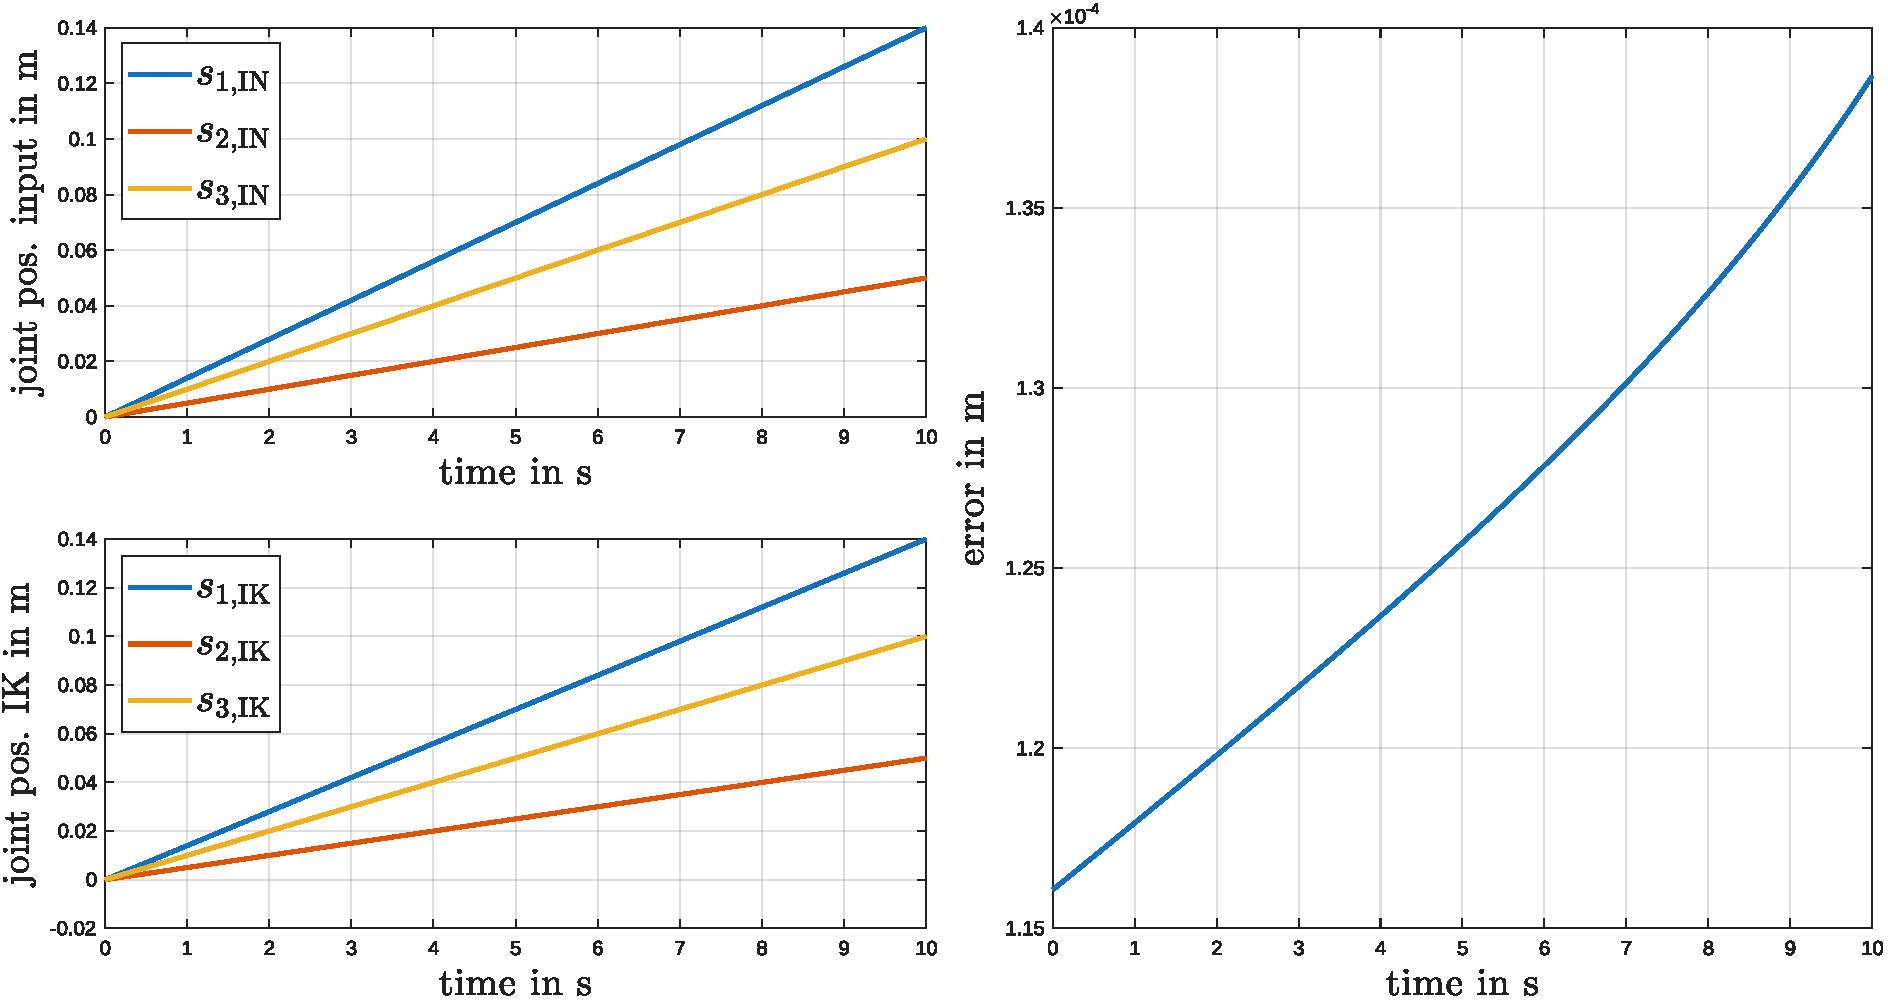
\includegraphics[width=1.0\linewidth]{cus_imgs/in_kin_verification}
	\caption[Plot of verification process for inverse kinematics]{Plot of Verification process for inverse kinematics. Left column: input joint position into Multibody model (MB) and output of inverse kinematics function (IK); right column: euclidean error of the two}
	\label{fig:inkinverification}
\end{figure}

It is apparent, that the inverse kinematics (IK) function yields the same results as the joint positions that were input into the simulation. The error, however, has a magnitude of $10^{-4}\,\si{\meter}$, which is larger than for forward kinematics.
% !TeX root = ../Main-Report.tex

\chapter{Joint Space Motion}

In this section, the process of oding joint space motions with the robot is documented. First, three waypoints are chosen inside of the workspace of the robot. They can be seen in table \ref{tab:jspace_waypoints}.

\begin{table}[H]
\centering
\caption{Chosen waypoints for trajectory planning}
\label{tab:jspace_waypoints}
\begin{tabular}{llll}
	Waypoint & $x$    & $y$    & $z$   \\ \hline
	$1$      & $0.0$  & $0.0$  & $0.4$ \\
	$2$      & $0.1$  & $0.1$  & $0.4$ \\
	$3$      & $-0.1$ & $-0.1$ & $0.4$ \\
	$4$      & $0.1$  & $-0.1$ & $0.4$ \\
	$5$      & $0.0$  & $0.0$  & $0.0$
\end{tabular}
\end{table}

Using the acceleration and velocity constraints that were given in the task, the synchronized velocity profile has been calculated in the file \textit{jspace\_trapz.m}. The outputs are time stamps and corresponding velocity values, which are then input into a Repeating table block in Simulink and fed into an integrator to receive the needed position information. As the simulation uses the vectors from the workspace, the script \textit{jspace\_trapz.m} needs to be run before the simulation.

\begin{figure}[H]
	\centering
	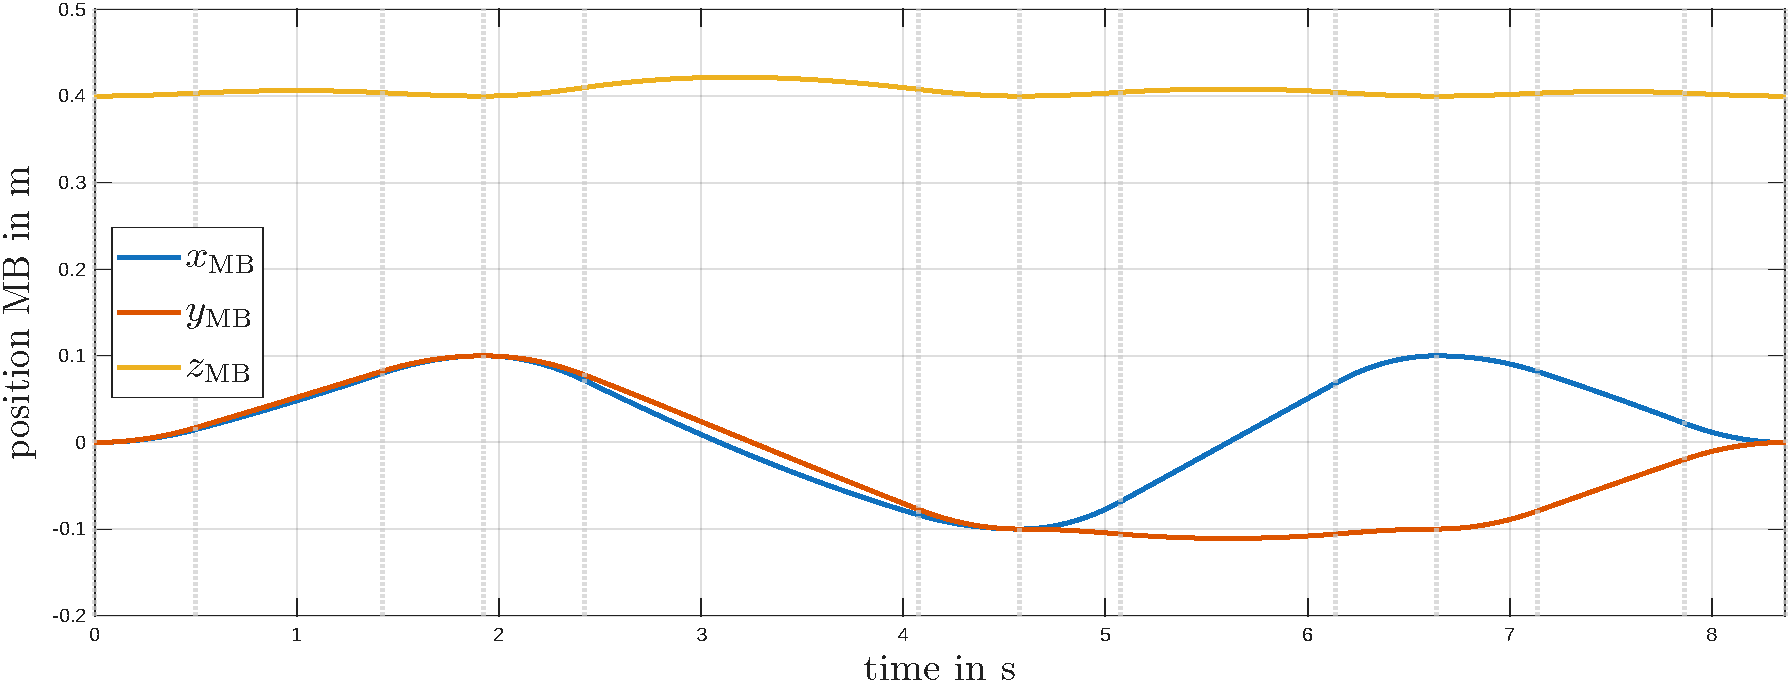
\includegraphics[width=1.0\linewidth]{cus_imgs/joint_trapz_xyz.pdf}
	\caption{$x$, $y$ and $z$ position of the end-effector for the trapezoidal velocity profile}
	\label{fig:jspace_trapz_xyz}
\end{figure}

Figure \ref{fig:jspace_trapz_xyz} shows the position of the end-effector of the robot when following the trapezoidal trajectory. The trajectory itself, with position, velocity and acceleration profile can be viewed in figure \ref{fig:jspace_trapz_traj}.

\begin{figure}[H]
	\centering
	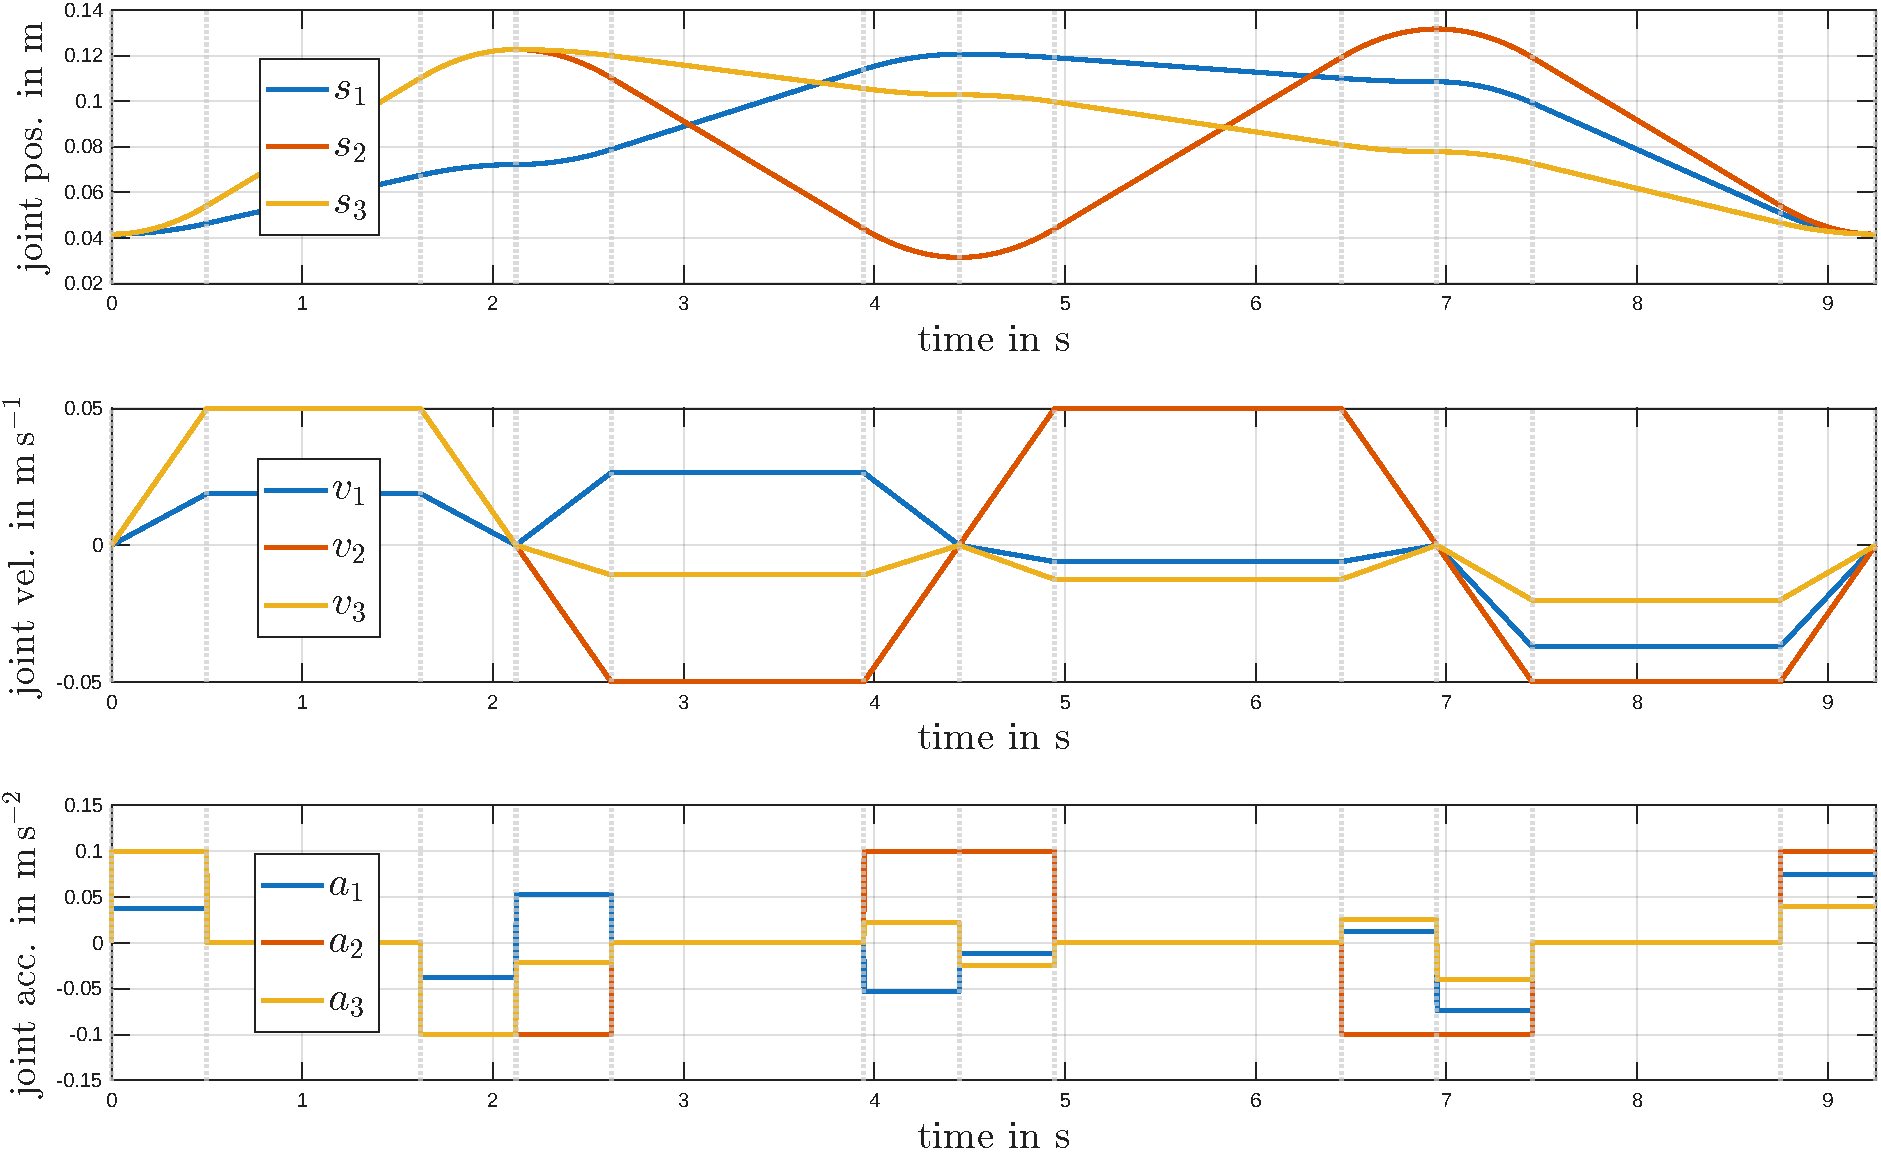
\includegraphics[width=1.0\linewidth]{cus_imgs/joint_trapz.pdf}
	\caption{Generated trajectory, including position, velocity and acceleration profiles}
	\label{fig:jspace_trapz_traj}
\end{figure}
% !TeX root = ../Main-Report.tex

\chapter{Task Space Motion}
This section document the implementation of movements in task space. 

\section{Trapezoidal trajectory in task space}

The same waypoints from the joint space motion have been used, which are visible in table \ref{tab:jspace_waypoints}. The maximum velocity of the end-effector was set to be $0.04\,\si{\meter\per\second}$, the maximum acceleration $0.07\,\si{\meter\per\square\second}$. The motion of the end-effector can be viewed in figure \ref{fig:tspace_trapz_traj}.

\begin{figure}[H]
	\centering
	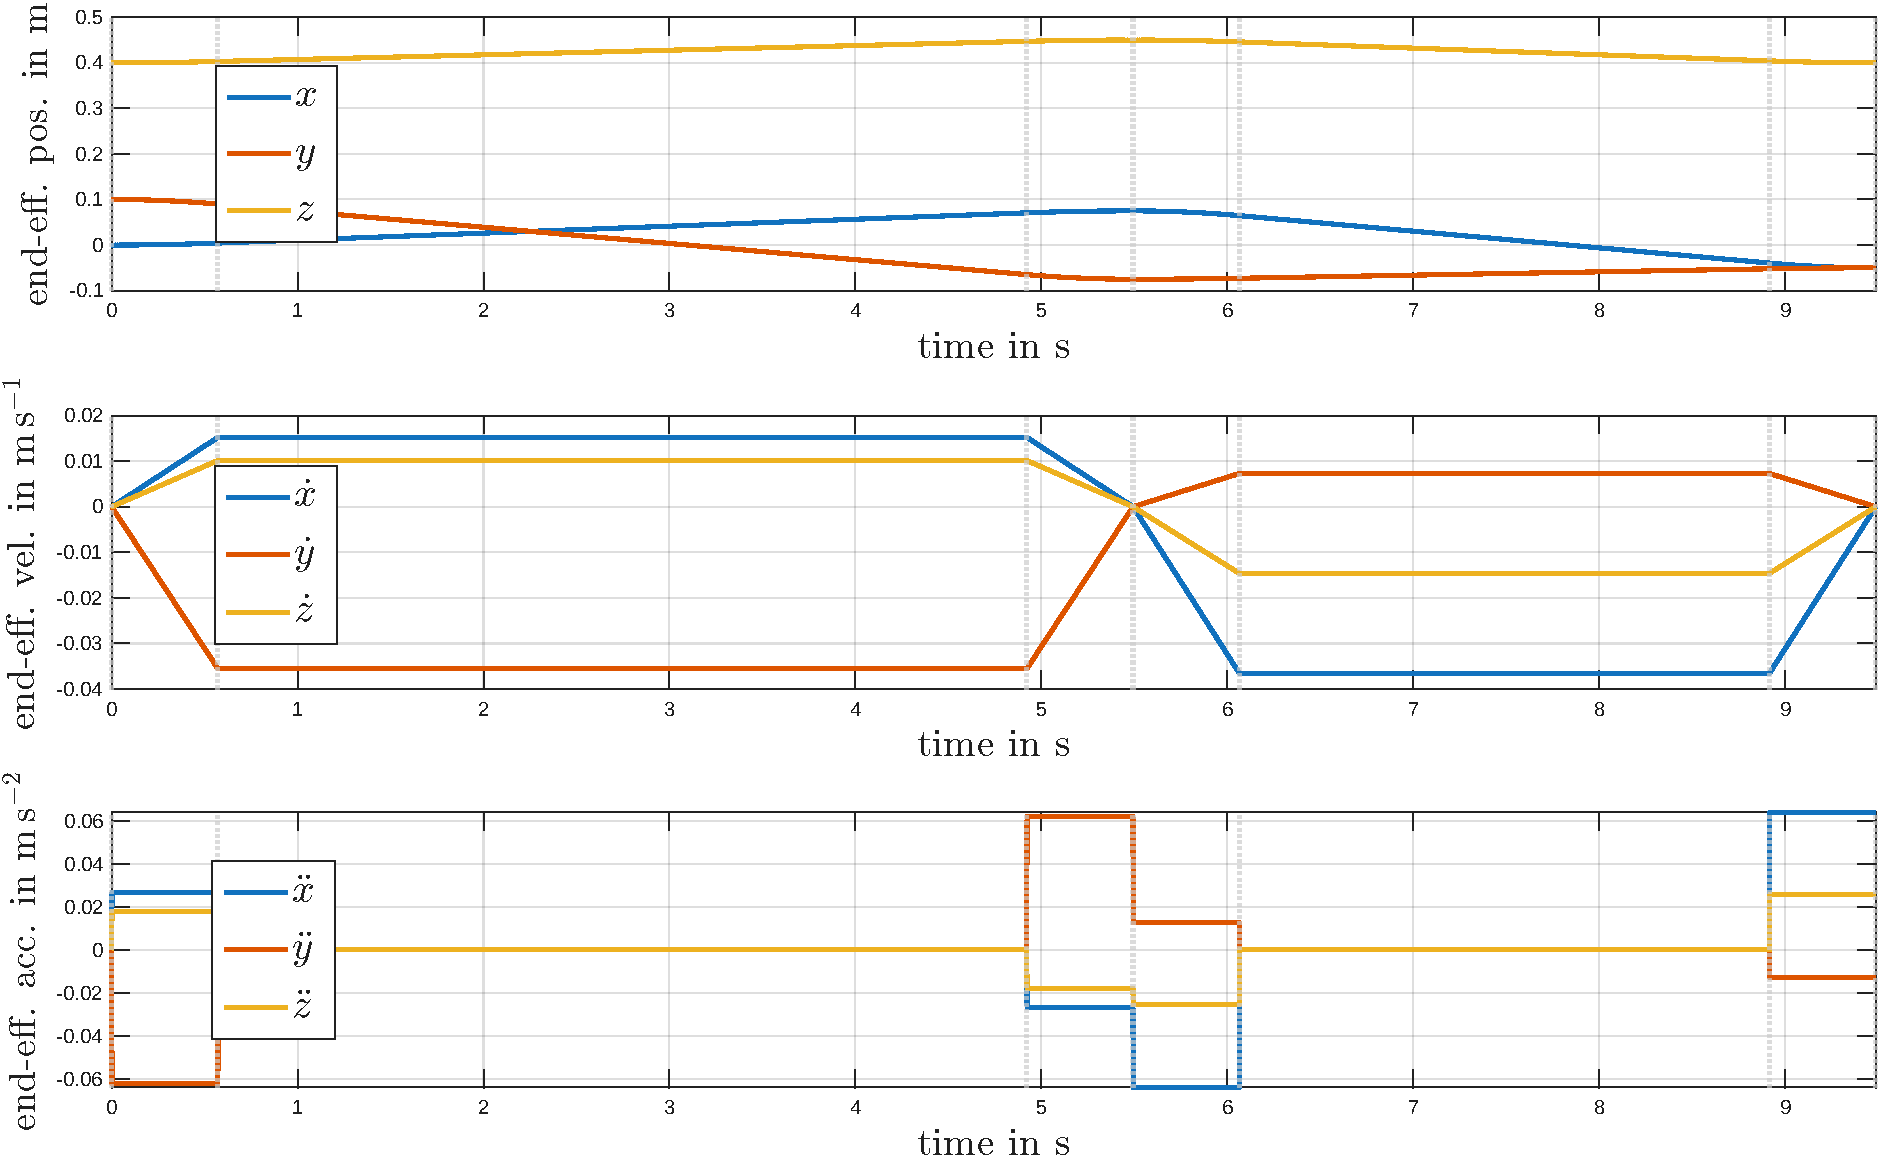
\includegraphics[width=1.0\linewidth]{cus_imgs/task_trapz.pdf}
	\caption{Position, velocity and acceleration of the end-effector for task space motion}
	\label{fig:tspace_trapz_traj}
\end{figure}

As expected, the end-effector moves in a straight line from point to point. The acceleration and velocity constraints are fulfilled.

\section{Double-S trajectory in task space}
Similar to the double-S velocity profile in task space, using a trapezoidal acceleration profile for task space trajectories make it possible to limit the jerk. In this case, the maximum jerk was set to $5\,\si{\meter\per\cubic\second}$.

\begin{figure}[H]
	\centering
	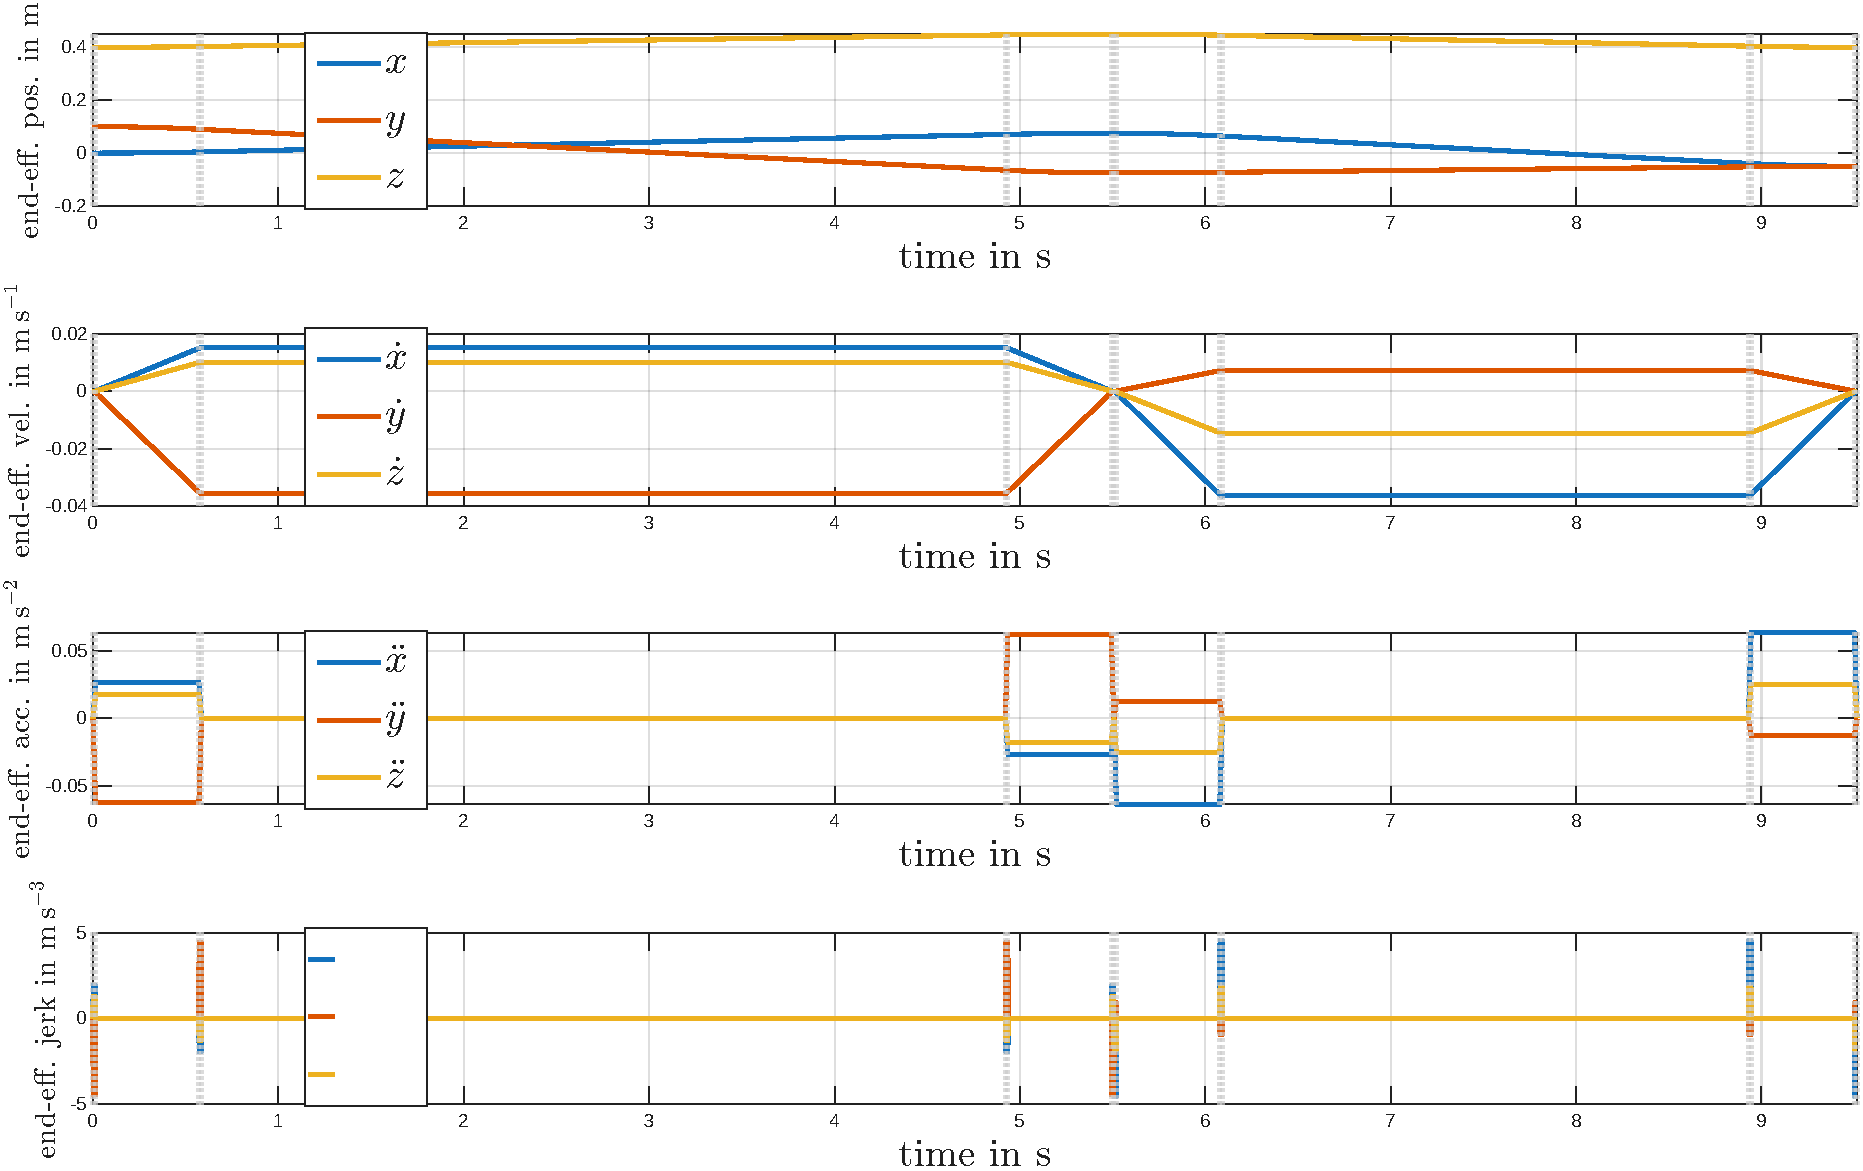
\includegraphics[width=1.0\linewidth]{cus_imgs/task_double_s.pdf}
	\caption{Double-S trajectory, including position, velocity, acceleration and jerk profiles in task space}
	\label{fig:tspace_ds_traj}
\end{figure}

As the jerk limit is relatively high, the double-S shape of the velocity of the end-effector is barely visible, but it is still there.


\section{Comparison joint and task space} \label{sec:comparison_jspace_tspace}

Compared to the joint space motion, the task space motion takes more time to execute within the constraints. A comparison of the joint velocities and accelerations for the trapezoidal velocity profiles for both can be viewed in figure \ref{fig:jspace_vs_tspace}.

\begin{figure}[H]
	\centering
	
\includegraphics[width=1.0\linewidth]{cus_imgs/joint_vs_task.pdf}
	\caption{Velocity and acceleration of the joints for joint and task space motion (trapezoidal)}
	\label{fig:jspace_vs_tspace}
\end{figure}

It is apparent that the joint velocities and accelerations in task space (right column) are much smaller than in joint space (left column). This is the cause of the motion taking significantly longer. The difference in the path that the end-effector takes in both motion modes can be viewed in figure \ref{fig:jspace_vs_tspace_motion}.

\begin{figure}[H]
	\centering
	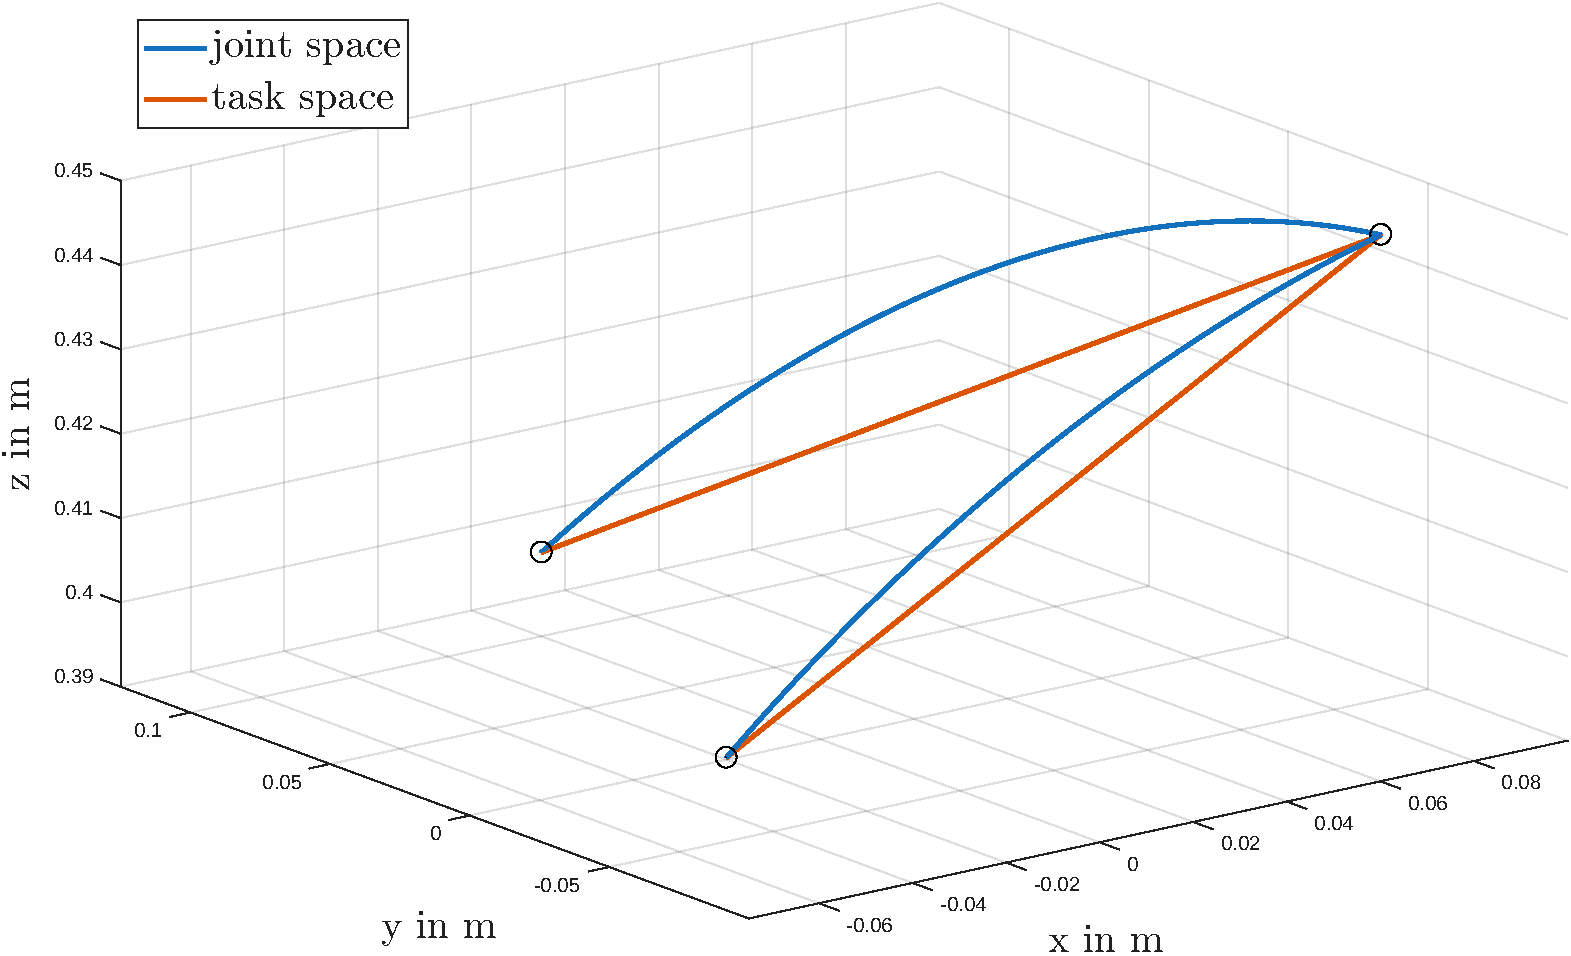
\includegraphics[width=0.9\linewidth]{cus_imgs/joint_vs_task_motion_3d.pdf}
	\caption{End-effector position in joint and task space}
	\label{fig:jspace_vs_tspace_motion}
\end{figure}

The Simulink setup used to fullfill these tasks (and parts of the next) can be seen in figure \ref{fig:joint_task_simulink}.

\begin{figure}[H]
	\centering
	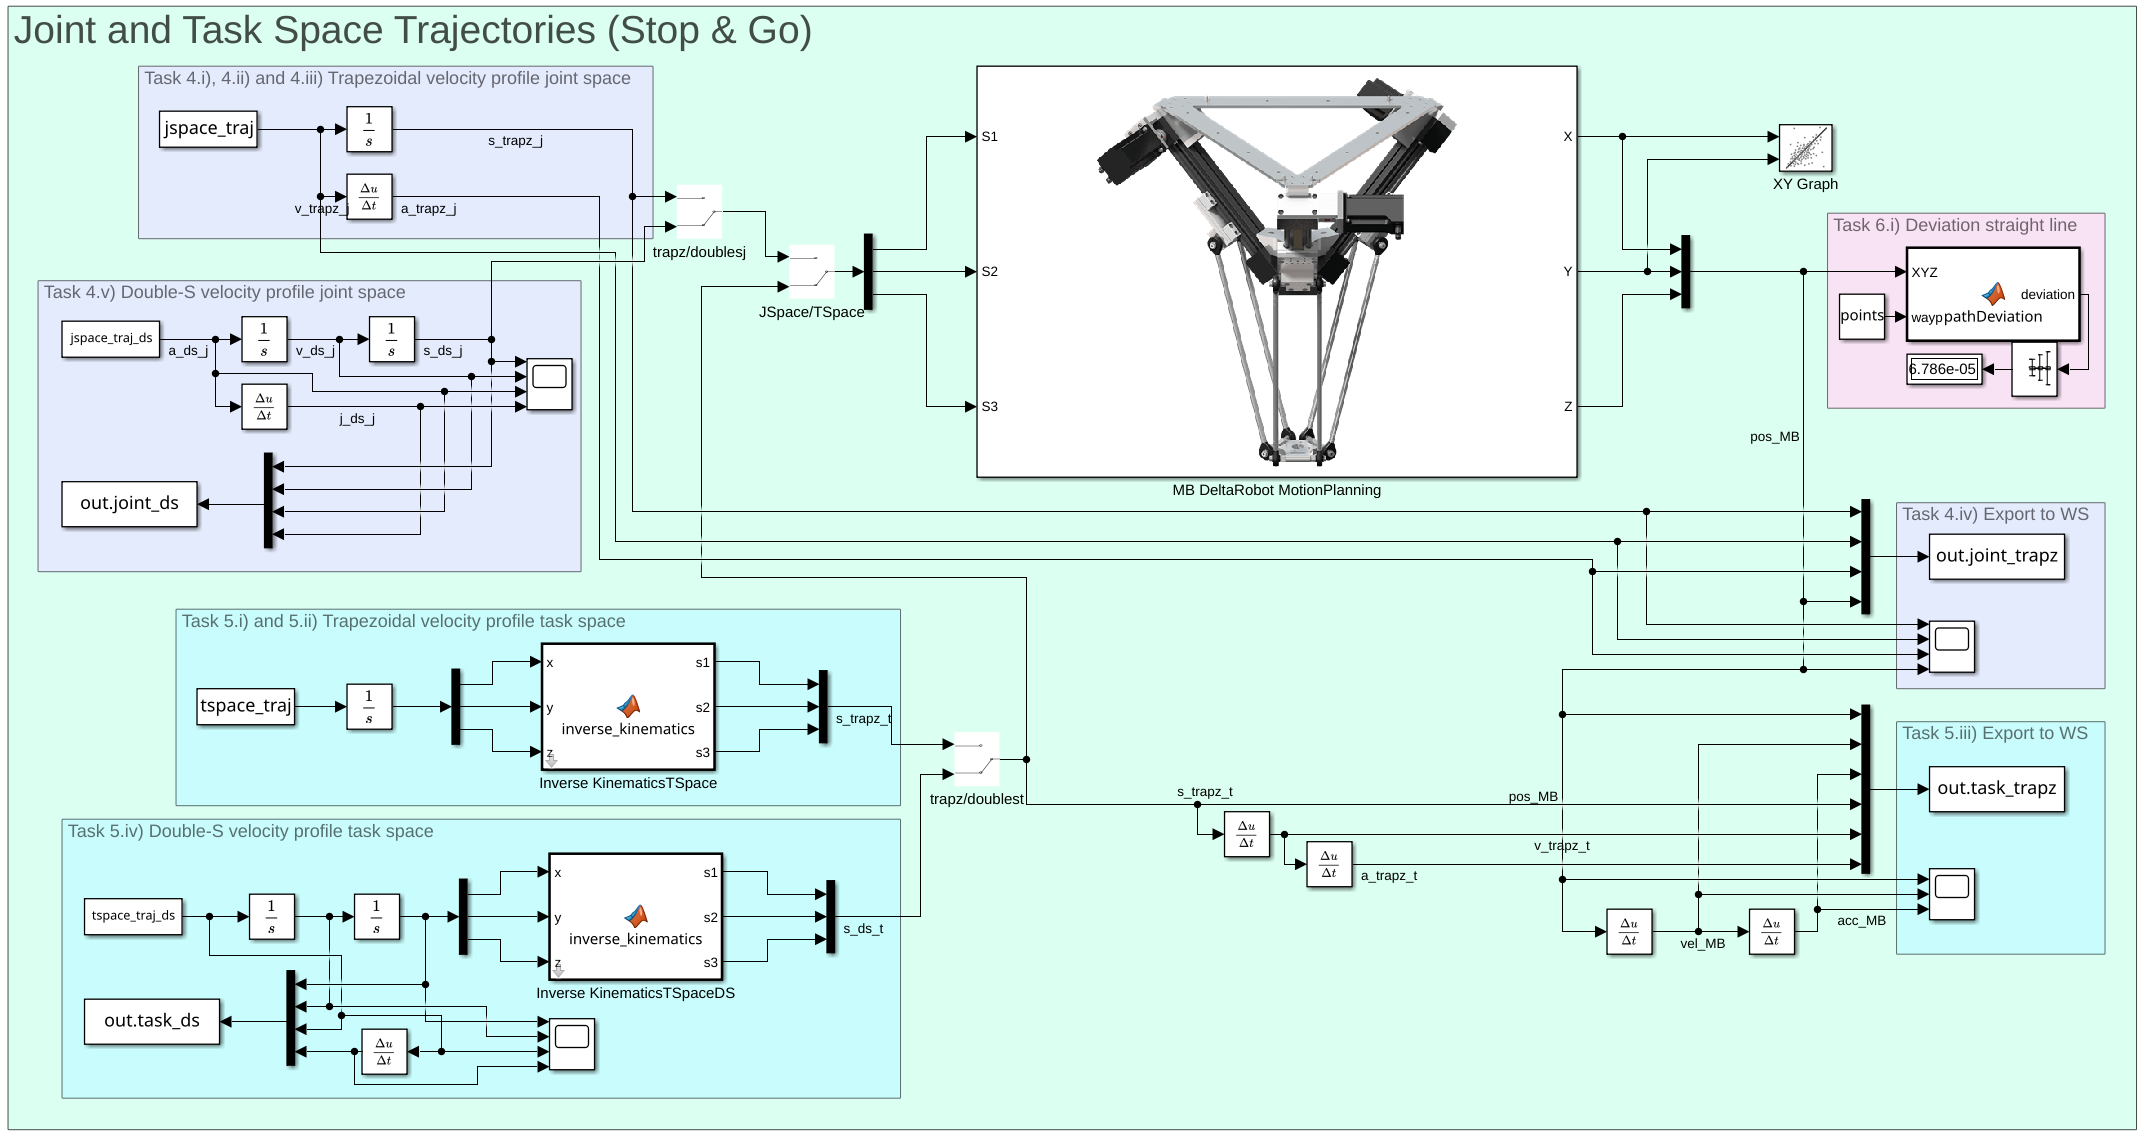
\includegraphics[width=1.0\linewidth]{cus_imgs/JSPACE_TSPACE_simulink.png}
	\caption{Simulink layout for joint and task space trajectories}
	\label{fig:joint_task_simulink}
\end{figure}
% !TeX root = ../Main-Report.tex

\chapter{Continuous Trajectory}
The enxt task was to implement a continuous trajectory between the chosen task space points from before(table \ref{tab:jspace_waypoints}), but without any full-stops at the via position. To achieve this, a cubic spline interpolation has been implemented. The joint position and velocites can be viewed in figure \ref{fig}

\begin{figure}[H]
	\centering
	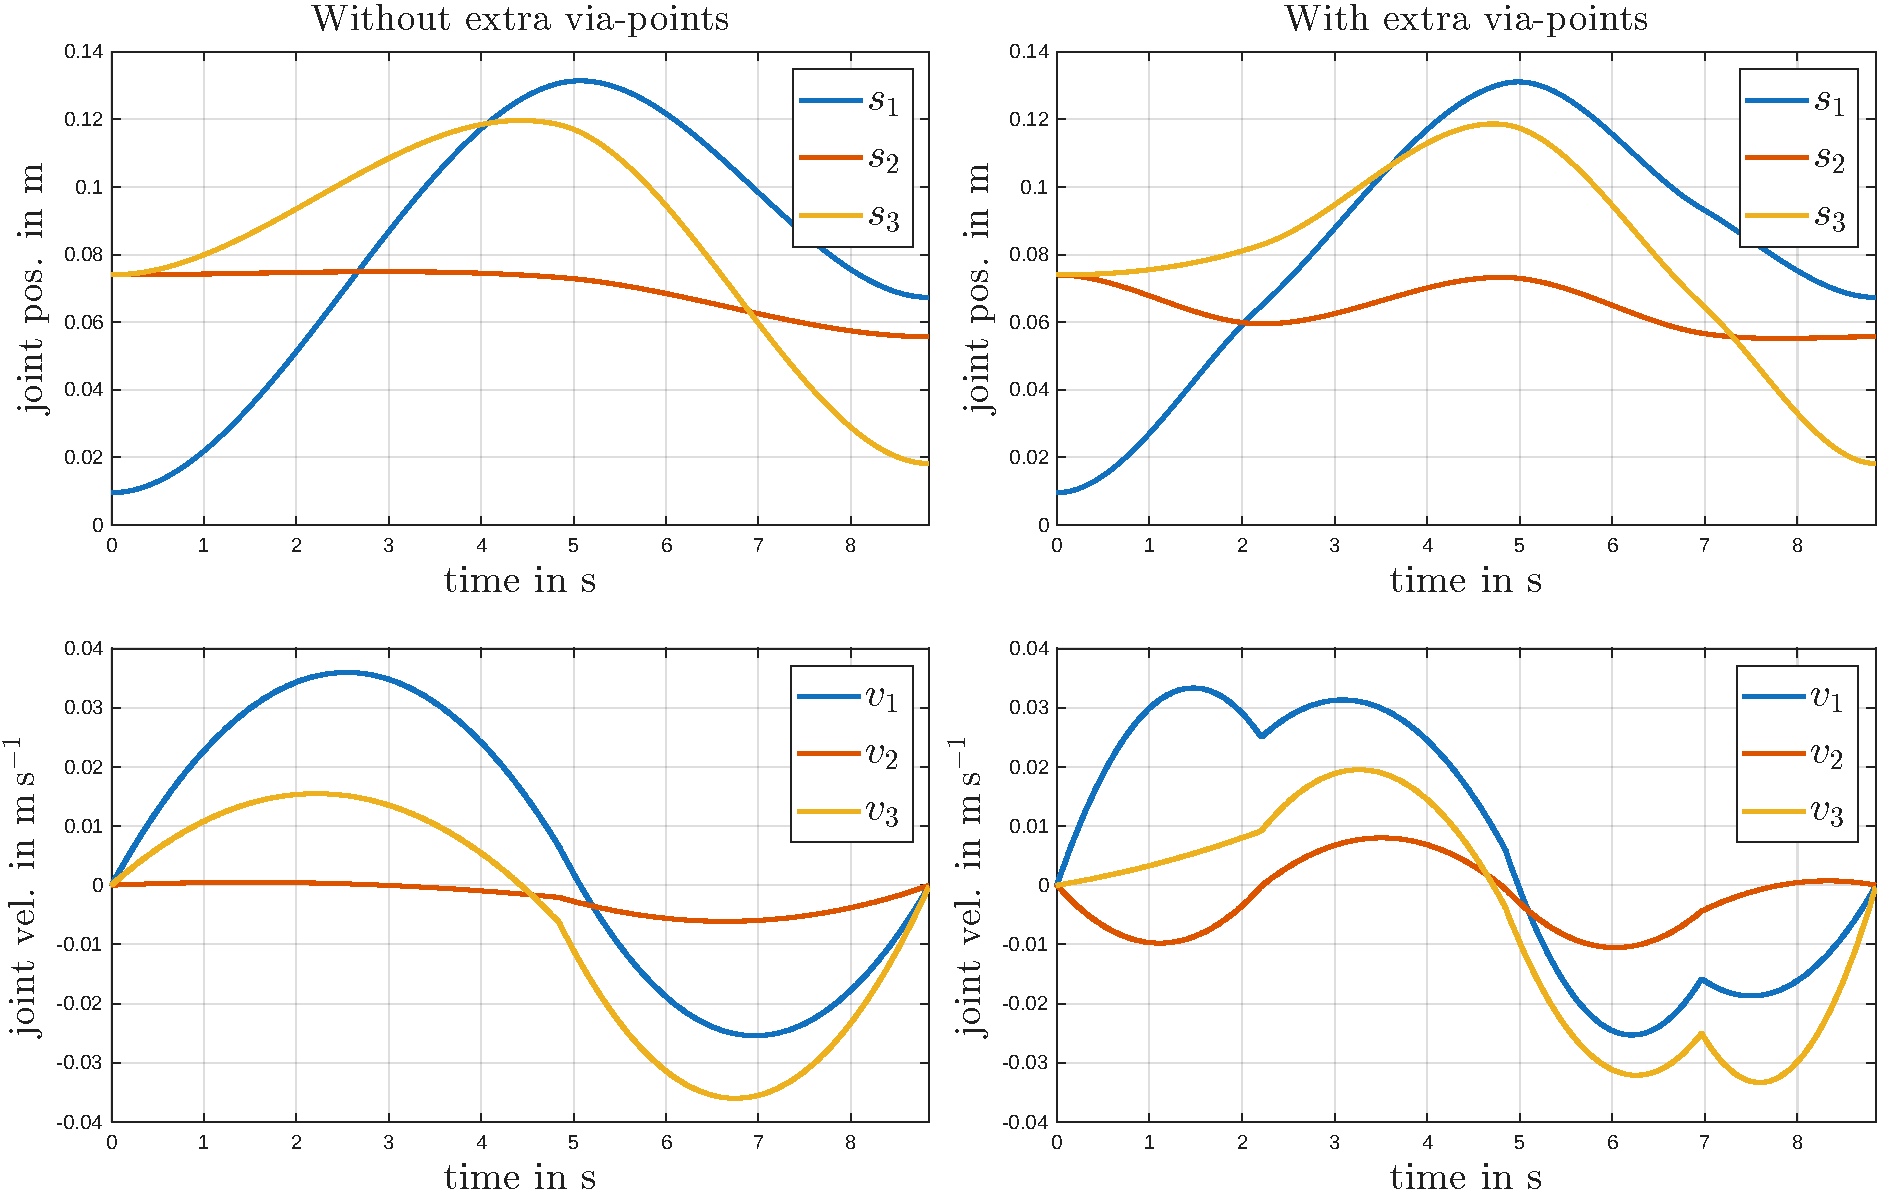
\includegraphics[width=1.0\linewidth]{cus_imgs/joint_con.pdf}
	\caption{Position and velocity of joints using a continuous trajectory, with and without extra via-points}
	\label{fig:jspace_con}
\end{figure}


\begin{figure}[H]
	\centering
	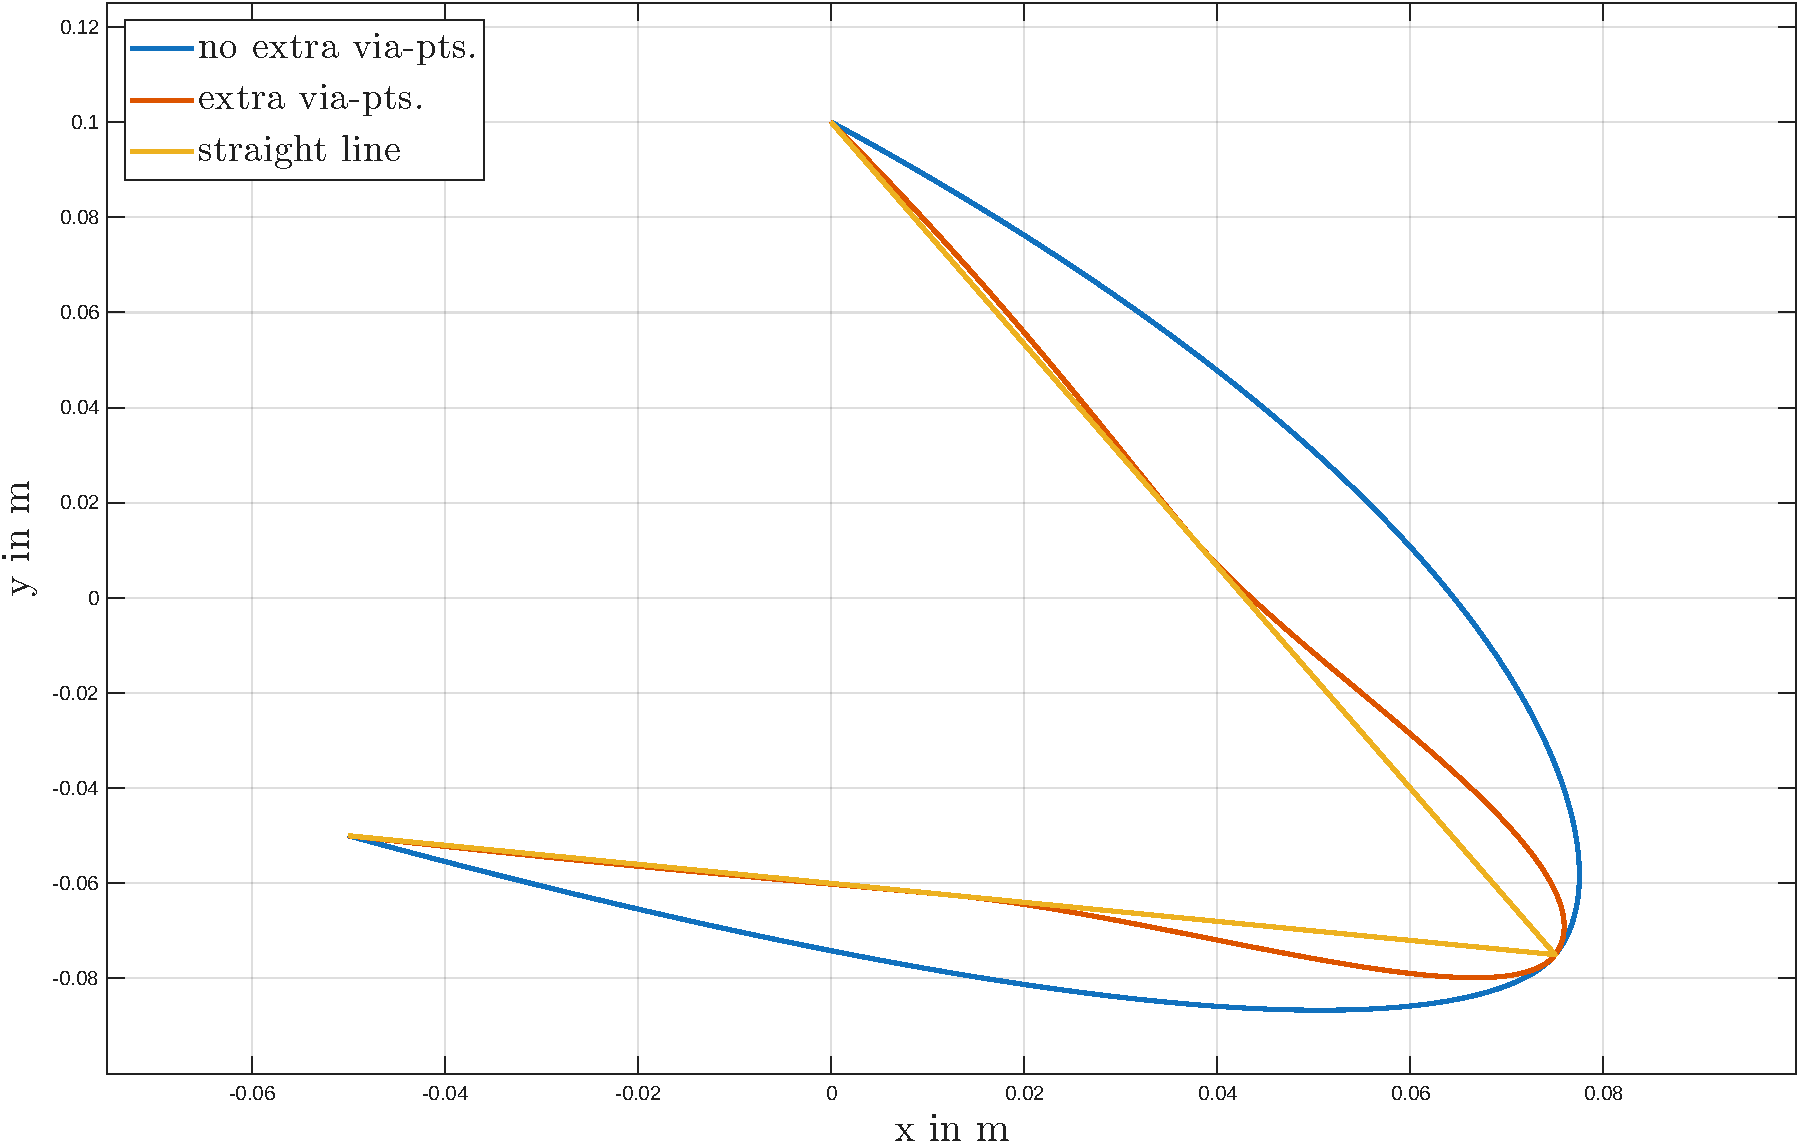
\includegraphics[width=1.0\linewidth]{cus_imgs/con_viapoints.pdf}
	\caption{End-effector $x$ and$y$ position with and without extra via-points}
	\label{fig:with_without_vias}
\end{figure}

% ---- 
% Add as many chapters as you see fit for your content. For easy legibility and for dynamic
% adjustment of content it would be suggested to write your files and place them similar to
% the aforementioned examples.

% REPORT POSTAMBLE ----------------------------------------------------------------------------

% ----
% In this section, please put all the thing you deem are necessary for the thesis but does have
% no substance as materials (i.e., technical drawings, patents, massive code bases).
% ----

\printbibliography

% \makeindex
% \printnomenclature
% \printglossaries

\end{document} % ##############################################################################
